\documentclass[10pt,spanish,a4paper,openany,notitlepage]{article}
\usepackage{etex}
%-------------------------------------Paquetes-----------------------------------------------------------------------
\usepackage[spanish,es-tabla]{babel}  	% Traduce los textos a castellano
\usepackage[utf8]{inputenc}	% Permite escribir directamente áéíóúñ
\usepackage{t1enc}            	% Agrega caracteres extendidos al font
\usepackage{amsmath} 		%Permite imprimir mas opciones matemáticas
\usepackage{graphicx}		%Permite agregar imagenes al informe
\usepackage{float} 		%Permite utilizar H para colocar las imagenes en un lugar especifico 
\usepackage{units}
\usepackage{circuitikz}
\usepackage{caption}
\usepackage{subcaption}
\usepackage{sidecap}
\usepackage{mathtools}
\usepackage{multirow} % Paquete para dividir las tablas en subtablas
\usepackage{booktabs} %estos 2 sirven para achicar la tabla
\usepackage{tabulary}
\usepackage{fancyhdr} % encabezado
\usepackage{textcomp} % para usar ° con el comando \textdegree
\usepackage{anysize}		%Permite modificar los margenes del documento
\usepackage{abstract} % paquete para el resumen del articulo
\usepackage{amssymb}
\usepackage{courier}
\usepackage{color}
\usepackage{listings}
\usepackage{pdfpages}



\definecolor{dkgreen}{rgb}{0,0.6,0}
\definecolor{gray}{rgb}{0.5,0.5,0.5}

\lstdefinelanguage
   [x64]{Assembler}     % add a "x64" dialect of Assembler
   [x86masm]{Assembler} % based on the "x86masm" dialect
   % with these extra keywords:
   	{
   	alsoletter={.\#},	
	morecomment=[l]{;},
    	morestring=[b]',
	morekeywords={[1],\#define,.org,main,ldi,rcall,ramend,_sfr_io_ADDR,spl,sph,
					lds,sts,clr,cpse,rjmp,cbi,sbi,cpi,breq,,ocr2,,eecr,eewe,eearh,
					eearl,eecr,eere,eedr,ddrb,portb,cpi,cp,brlo,breq,sbrs,sbis,lsr,
					brsh,sbrc,sbic,pinb,.byte,.section,.text,.data,.eeprom,.end,
					lo8,hi8,.global,\#include,r1,r2,r3,r4,r5,r6,r7,r8,r9,10,r11,r12,
					r13,r14,r15,r16,r17,r18,r19,r20,r21,r22,r23,r24,r25,r26,r27,
					r28,r29,r30,r31,r32,r33,r34}
  	} % etc.

\lstset{language=[x64]Assembler,
   keywordstyle=\bf\color{blue},
   commentstyle=\it\color{dkgreen},
   stringstyle=\color{gray},
   numbers=left,
   numberstyle=\tiny\color{black},
   stepnumber=2,
   numbersep=8pt,
   backgroundcolor=\color{white},
   tabsize=4,
   showspaces=false,
   showstringspaces=false,
   extendedchars=\true,
	inputencoding=utf8}

% todo lo que sigue es para poner links que se les pueda hacer click
\usepackage{xcolor}
\usepackage[normalem]{ulem}
\usepackage{hyperref}
\hypersetup{colorlinks,urlcolor=blue}



%---------------------------------------Configuraciones de pagina----------------------------------------------
\marginsize{2.5cm}{2.5cm}{1cm}{1cm}

\pagestyle{fancy}
\fancyhf{}
\lhead{
66.09 - \textsc{Laboratorio de Microcomputadoras}\\ 
1\textsuperscript{er} Cuatrimestre de 2015
}
\rhead{
\includegraphics[width=3cm]{imagenes/FIUBA_ALTA.jpg}}
\rfoot{Página \thepage}

%---------------------------------------Definiciones propias---------------------------------------------------------
\newcommand{\oiint}{\displaystyle\bigcirc\!\!\!\!\!\!\!\!\int\!\!\!\!\!\int} %Integral doble cerrada

\DeclarePairedDelimiter\abs{\lvert}{\rvert}%
\DeclarePairedDelimiter\norm{\lVert}{\rVert}%
% Swap the definition of \abs* and \norm*, so that \abs
% and \norm resizes the size of the brackets, and the 
% starred version does not.
\makeatletter
\let\oldabs\abs
\def\abs{\@ifstar{\oldabs}{\oldabs*}}
%
\let\oldnorm\norm
\def\norm{\@ifstar{\oldnorm}{\oldnorm*}}
\makeatother
%--------------------------------------------------------------------------------------------------------------------------------


\makeatletter
\let\ps@plain\ps@fancy 
\makeatother

% lo siguiente es para borrar el titulo del resumen y que no ocupe espacio:
 \AtBeginDocument{%
 \renewcommand{\abstractname}{}%
 }
\renewcommand{\absnamepos}{empty} % originally center
 

\begin{document}


\begin{titlepage}
\begin{center}

\includegraphics[scale=0.5]{imagenes/FIUBA_ALTA.jpg}\\
\large{Laboratorio de Microcomputadoras  -  66.09}
\vspace{1cm}\\
\Huge{Dispositivo Autorregulador de la Percepción Térmica Corporal}\\
\vspace{7mm}
\normalsize
\begin{tabular}{|c|c|c|c|c|c|c|c|c|c|c|c|}
\hline
\multicolumn{3}{|c|}{Profesor:}  & \multicolumn{9}{|c|}{Ing. Guillermo Campiglio}\\
\hline
\multicolumn{3}{|c|}{Cuatrimestre/Año:}  & \multicolumn{9}{|c|}{1º/2015}\\
\hline
\multicolumn{3}{|c|}{Turno de las clases prácticas}  & \multicolumn{9}{|c|}{miercoles}\\
\hline
\multicolumn{3}{|c|}{Jefe de trabajos prácticos:}  & \multicolumn{9}{|c|}{Ricardo Arias}\\
\hline
\multicolumn{3}{|c|}{Docente guía:}  & \multicolumn{9}{|c|}{Ricardo Arias}\\
\hline
\multicolumn{12}{|c|}{}\\
\hline
\multicolumn{3}{|c|}{Autores}  & \multicolumn{9}{|c|}{Seguimiento del proyecto}\\
\hline
Gaston & Martinez & 91383 & \hspace{4mm} & \hspace{4mm} & \hspace{4mm} & \hspace{4mm} &\hspace{4mm} &\hspace{4mm} &\hspace{4mm} &\hspace{4mm} &\hspace{4mm} \\
\hline
Matías & Vázquez  & 91523& \hspace{4mm} & \hspace{4mm} & \hspace{4mm} & \hspace{4mm} &\hspace{4mm} &\hspace{4mm} &\hspace{4mm} &\hspace{4mm} &\hspace{4mm} \\
\hline
\end{tabular}

\vspace{9mm}
{\bf Observaciones:}\\
..........................................................................................................\\
..........................................................................................................\\
..........................................................................................................\\
..........................................................................................................\\
..........................................................................................................\\
..........................................................................................................\\
..........................................................................................................\\
..........................................................................................................\\
..........................................................................................................\\

\vspace{10mm}

\begin{tabular}{|c|c|c|c|c|}
\hline
\multicolumn{3}{|c|}{Fecha de aprobación} & \hspace{10mm} & Firma J.T.P\\
\hline
\hspace{10mm} & \hspace{10mm} & \hspace{10mm} &&\\
\hline
\end{tabular}
\-\\
\vspace{10mm}
\begin{tabular}{|c|c|}
\hline
\multicolumn{2}{|c|}{Coloquio}\\
\hline
Nota final&\hspace{2cm} \\
\hline
Firma profesor&\hspace{2cm} \\
\hline
\end{tabular}
\end{center}
\end{titlepage}
\newpage


\tableofcontents
\newpage

\section{Objetivos}
Se diseñó e implementó una pulsera térmica que regula la temperatura
de la muñeca del usuario. Se utiliza un módulo termoeléctrico para enviar
variaciones de calor o frío a fin de modificar
la percepción térmica del cuerpo.

Su función es generar pulsos de frío o calor, de manera de generar una sensación de 
confort para una persona en condiciones donde la temperatura es muy alta 
o muy baja respectivamente.
Está basado en el proyecto \emph{Wristify} \cite{embrlabs} ganador del concurso de Intel: 
\emph{Make It Wearable} \cite{Make It Wearable}.

\subsection{Diagrama de Bloques}

\begin{figure}[H] %[h] para here [b] para bottom [t] para top [H]+float para aqui si o si
\begin{center}
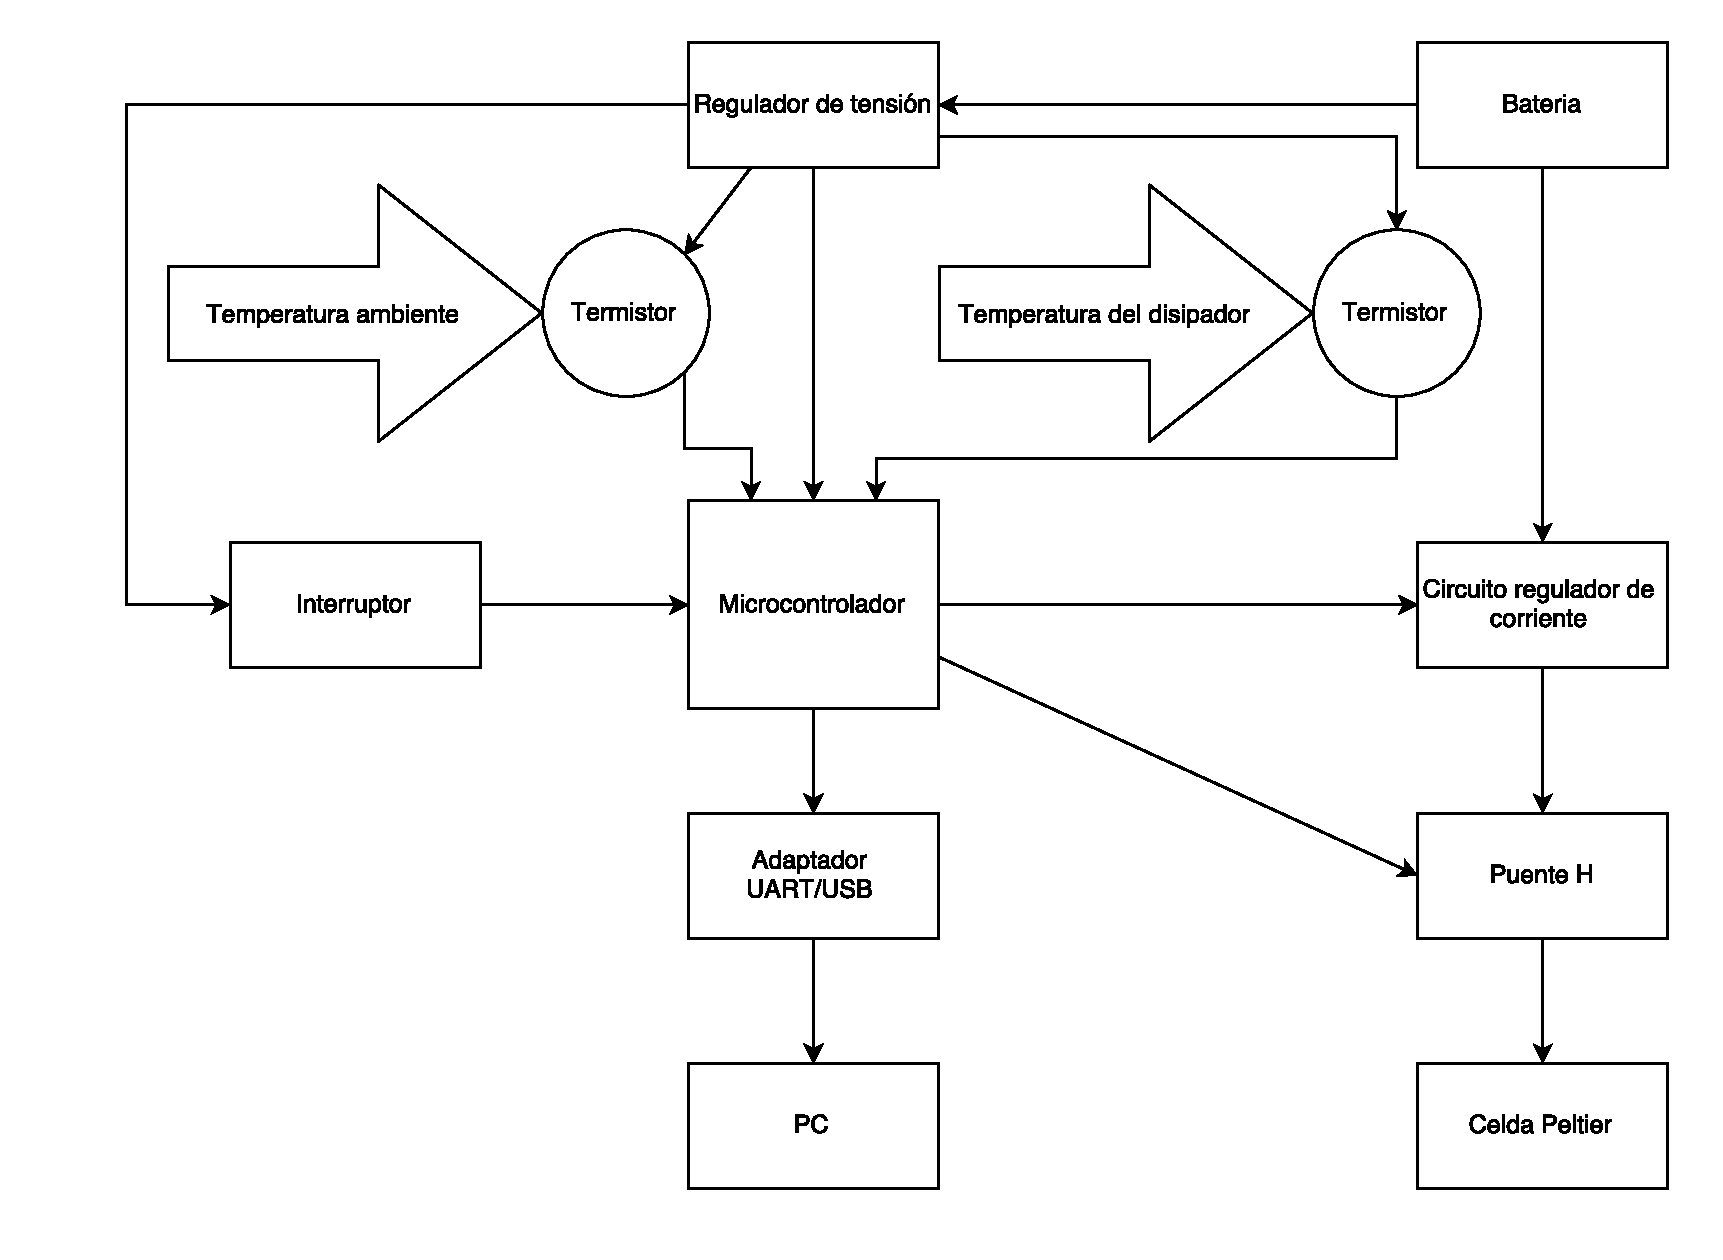
\includegraphics[scale=0.55]{./imagenes/diagrama_de_bloques.pdf}
\caption{Diagrama de bloques}
 \label{fig:diag_bloques}
\end{center}
\end{figure}



\subsection{Diagrama de Flujo}

\begin{figure}[H] %[h] para here [b] para bottom [t] para top [H]+float para aqui si o si
\begin{center}
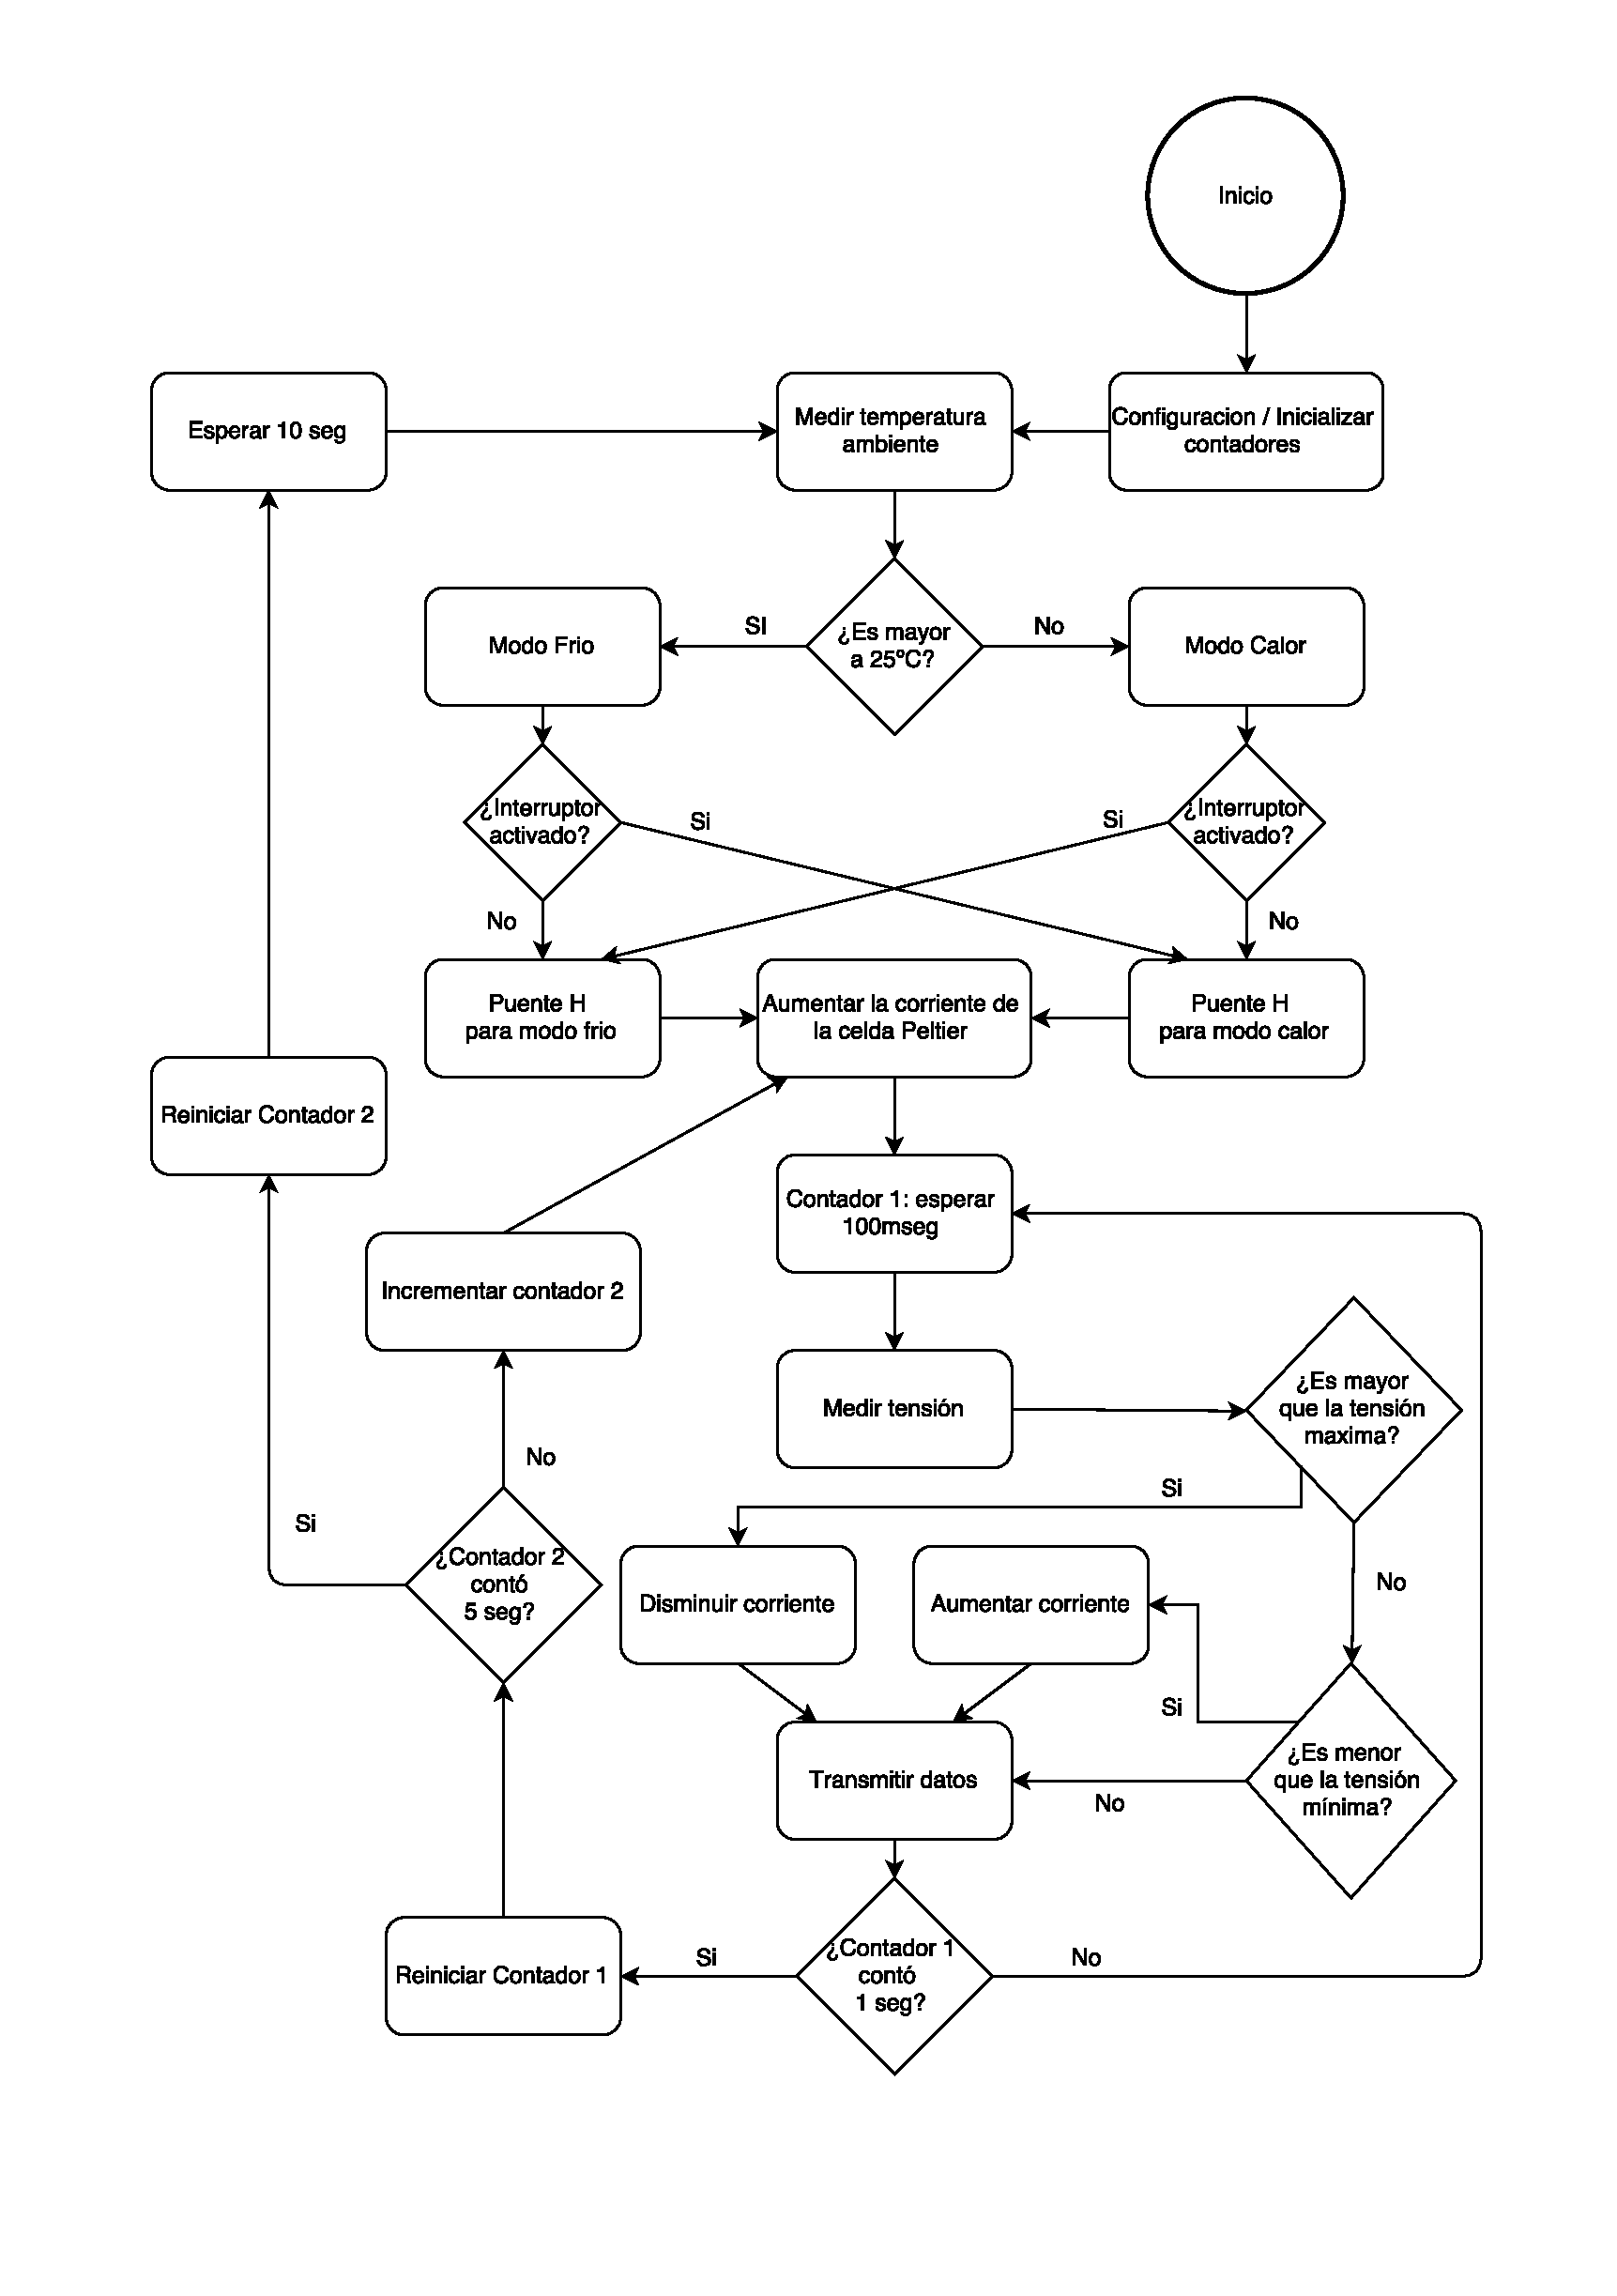
\includegraphics[scale=0.55]{./imagenes/diagrama_de_flujo.pdf}
\caption{Diagrama de flujo del proceso}
 \label{fig:diag_flujo}
\end{center}
\end{figure}


\subsection{Especificaciones}

El dispositivo utiliza una celda Peltier para enviar pulsos de calor
o frío. De forma que se logre una diferencia de temperatura mayor a $0,4\, \unit{^oC/seg.}$
durante 5 segundos y durante los siguientes 10 segundos entra
en estado de espera, para luego volver a iniciar el ciclo. 

Cuenta con un termistor para medir la temperatura ambiente
y analizar si deberá enviar pulsos frios o calidos.

Finalmente deberá controlar que se cumpla el ciclo en base a la corriente
que circulará por la celda Peltier.

\subsubsection{Componentes}

A continuación se lista la función de cada componente.

\begin{itemize}
\item{Celda Peltier:} Realiza los cambios de temperatura en la muñeca del usuario.
\item{Circuito regulador de corriente:} Regula la corriente suministrada
a la celda peltier.
\item{Puente H:} Invierte la polaridad de la celda Peltier, para así poder
alternar entre modo frío o modo calor.
\item{Disipador:} La celda Peltier contará con un disipador para mantener
la temperatura de una de sus caras a un valor cercano a la temperatura
ambiente.
\item{Termistores:} Cuenta con dos termistores. Uno para medir la
temperatura ambiente y en base a esta decidir el modo de trabajo, frío
o calor. El segundo termistor medirá la temperatura del disipador conectado
a la celda Peltier para poder realizar una estimación de la temperatura
de la celda.
\item{Salida de puerto serie:} Sirve para poder monitorear en una 
computadora la temperatura de la placa.
\item{Adaptador UART-USB:} Sirve para recibir los datos enviados desde
el microcontrolador en una PC a través del puerto USB.
\item{Bateria:} Suministra la corriente necesaria a la celda Peltier y 
 proporcionará alimentación a todos los dispositivos utilizados.
\item{Interruptor:} Para poder invertir el estado de trabajo, de frío a calor 
y viceversa.
\item{Controlador:} Se utilizara un microcontrolador AVR. Es
el encargado de obtener las temperaturas de los termistores para definir
el modo de trabajo y autorregular la corriente de la celda Peltier mediante
el circuito regulador de corriente.
\end{itemize}

\section{Diseño}

\subsection{Esquematico}


\begin{figure}[H] %[h] para here [b] para bottom [t] para top [H]+float para aqui si o si
\begin{center}
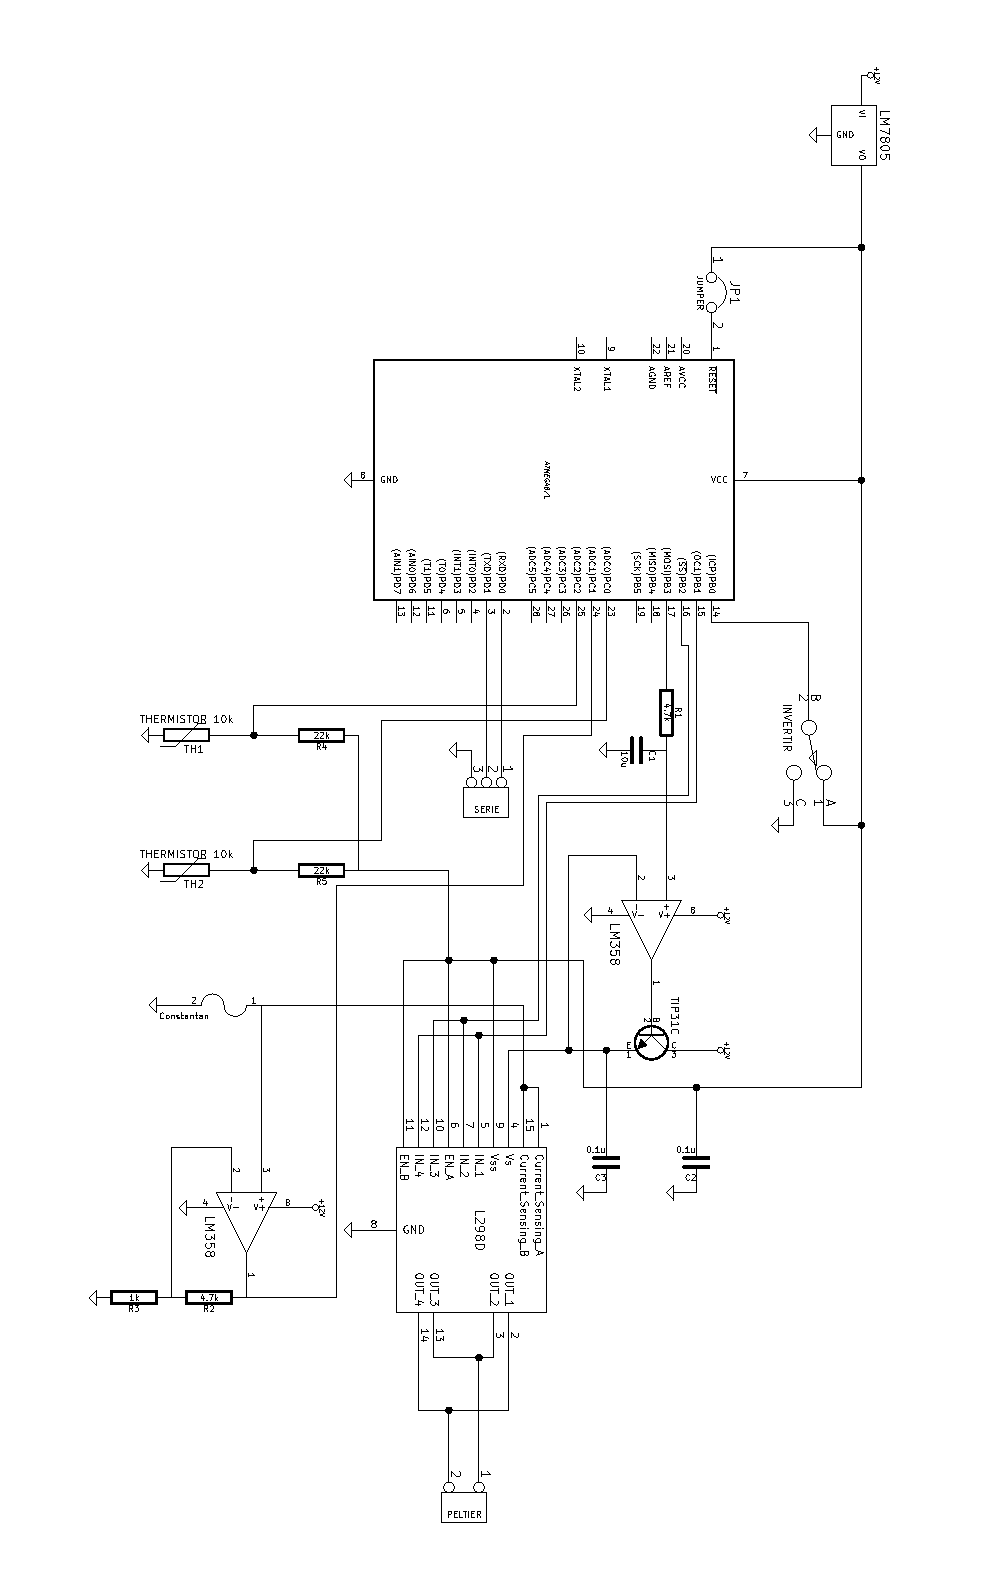
\includegraphics[scale=0.89, angle=-90]{../circuitos/esquematico.pdf}
\caption{Diagrama esquemático}
 \label{fig:esquematico}
\end{center}
\end{figure}

\subsection{Componentes}

\begin{itemize}
\item{Celda Peltier:} Celda peltier de $10\, \unit{W}$ y $15\, \unit{mm}$x$15\,\unit{mm}$ 
\item{LM7805:} Regulador de tensión para habilitar el puente H, alimentar
el microcontrolador y suministrarle tensión constante a las resistencias conectadas
en serie a los termistores.
\item{Interruptor:} Interruptor para activar la inversión de la polaridad.
\item{Resistencias:}
	\begin{itemize}
	\item Dos resiststencias de $4.7\,\unit{k\Omega}$
	\item Dos resiststencias de $22.0\,\unit{k\Omega}$
	\item Una resistencia de $1.0\,\unit{k\Omega}$
	\end{itemize}
\item{Capacitores:} 
	\begin{itemize}
	\item 1 capacitor de \unit{10\, \unit{$\mu$F}} para generar
	tensión constante del PWM recibido.
	\item 4 capacitores de \unit{0.1\, \unit{$\mu$F}} Conectados en paralelo
	a las alimentaciones del puente H, recomendados por el fabricante. 
	\end{itemize}
\item{LM358:} Dos amplificadores operacionales. Uno para suministrar corriente
a la base del NPN y el segundo para amplificar la tensión leída del constantán. 
\item{TIP31C:} Transistor de potencia NPN, utilizado para regular la corriente.
\item{L298D:} Puente H utilizado para invertir la polaridad de la celda Peltier
\item{Constantán:} alambre de $2\, \unit{cm}$ ($0.5\, \unit{mm}$ de diámetro) utilizado para sensar la corriente generada.
\item{Bateria:} de $12\, \unit{V}$ y $2.9\, \unit{Ah}$
\item{Pines:}
	\begin{itemize}
	\item 3 pines para el puerto serie.
	\item 2 pines para el reseteo del microcontrolador.
	\item 2 pines para conectar la celda peltier al circuito.
	\end{itemize}
\item{Termistores:} Dos termistores NTC de $10\, \unit{k\Omega}$
\end{itemize}

\subsection{Regulador de Corriente con Puente H}

Se utilizó un regulador de corriente controlado por un PWM como se muestra
en la figura \ref{fig:reg_corriente}

\begin{figure}[H] %[h] para here [b] para bottom [t] para top [H]+float para aqui si o si
\begin{center}
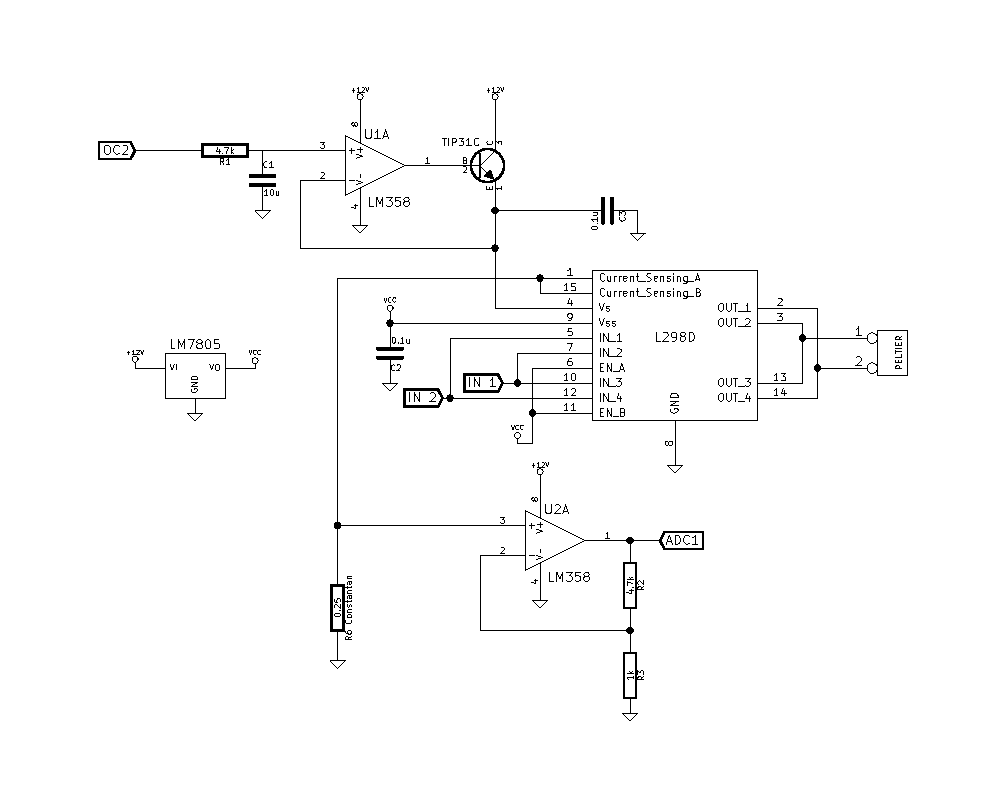
\includegraphics[scale=1]{../circuitos/regulador_corriente.pdf}
\caption{Regulador de Corriente}
 \label{fig:reg_corriente}
\end{center}
\end{figure}

El circuito RC filtra la señal del PWM generado por el
microcontrolador. Presentando el valor medio en la entrada no inversora del LM358 U1A,
cuya salida regulará la corriente suministrada a la
base del transistor NPN por el amplificador operacional, generando una corriente
constante entre el colector y el emisor del transistor.

Se optó por utilizar un L298D para el puente H ya que cuenta en un mismo
integrado con dos puentes H que soportan $2\, \unit{A}$ de corriente. 
Conectados en paralelo como se muestra en la figura \ref{fig:reg_corriente} 
se puede duplicar dicha corriente máxima para que soporte hasta $4\, \unit{A}$ de corriente.

La corriente que circula por la celda se mida con una resistencia hecha con
alambre constatán. La tensión que cae sobre este es amplificada por el LM358 U2A.
Para que la tensión de salida varíe entre $0\, \unit{V}$ y $2.56\, \unit{V}$
y sea leído por el microcontrolador.

Las resistencias del amplificador U2A se obtuvieron considerando que para
la corriente máxima registrada de $1.75\, \unit{A}$, la salida no supere los $2.56\, \unit{V}$.
Siendo de  $0.25\, \unit{\Omega}$ la resistencia del alambre constantan .

La tensión de salida se obtiene mediante:

\begin{equation}
V_{ADC1} = R_{constantan} I_{MAX} \frac{R_3 + R_2}{R_3}
\label{eq:tension_salida}
\end{equation}

Luego fijando $R_3 = 1\, \unit{k\Omega}$ y $R_2 = 4.7\, \unit{k\Omega}$
se verificó que la tensión no supere los $2.56\, \unit{V}$:

\[ \displaystyle V_{ADC1} = 0.25\, \unit{\Omega}\ 1.75\, \unit{A} \frac{1\, \unit{k\Omega} + 4.7\, \unit{k\Omega}}{1\, \unit{k\Omega}} = 2.49 \unit{V} < 2.56 \unit{V} \]

\subsection{Medición de las temperaturas}

Se utilizaron dos termistores. Uno para medir la temperatura ambiente y 
otro para la temperatura del disipador conectado a la celda Peltier para
poder estimar la temperatura a la que se encuentra la celda.
Ambos termistores están conectados de la misma manera como se indica a continuación.

Se utilizó un divisor resistivo para medir la tensión en los termistores y 
poder obtener la temperatura utilizando tablas con la relación entre
la tensión leída y la temperatura a la que se encuentra.
Se obtuvieron las resistencias a conectar en serie con los termistores de
forma que la tensión máxima no supere los $2.56\, \unit{V}$

\begin{figure}[H] %[h] para here [b] para bottom [t] para top [H]+float para aqui si o si
\begin{center}
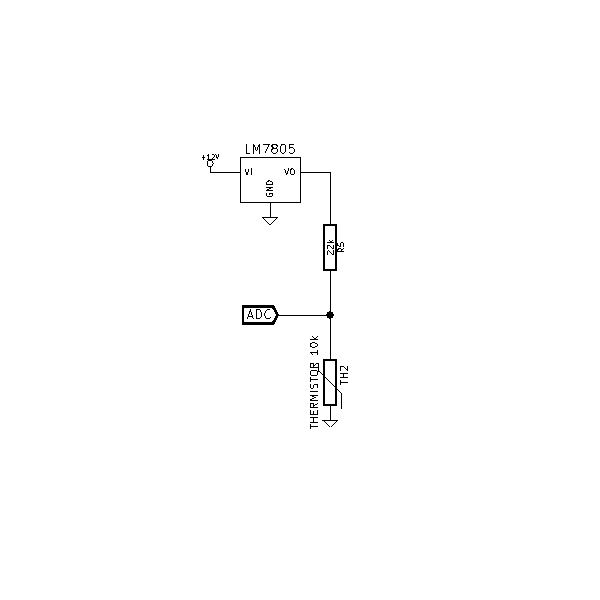
\includegraphics[scale=1.25]{../circuitos/temperatura.pdf}
\caption{Divisor de tensión de los termistores}
 \label{fig:temperatura}
\end{center}
\end{figure}

\begin{equation}
V_{termistor} = 5\, \unit{V} \frac{R_{termistor}}{R_{termistor}+R_{serie}}
\label{eq:tension_termistor}
\end{equation}

Finalmente se eligió una resistencia de $R_{serie} = 22\, \unit{k\Omega}$
para $R_4$ y $R_5$ verificando que la tensión en los termistores no supere
la tensión de referencia del ADC del microcontrolador para la resistencia
máxima registrada en los termistores a $R_{0\,\unit{^oC}} = 15\, \unit{k\Omega}$ :

\[ \displaystyle V_{termistor} = 5\, \unit{V} \frac{15\, \unit{k\Omega}}{15\, \unit{k\Omega}+22\, \unit{k\Omega}} = 2\, \unit{V}\]

\subsection{Interruptor selector de modo}

La salida del interruptor es recibida por el microcontrolador, para en 
el siguiente ciclo invertir la polaridad de la celda Peltier mediante el puente H y
evitar un cambio brusco de corriente en la celda Peltier.

El interruptor invertirá el modo de trabajo actual. En caso de encontrarse el dispositivo a temperaturas ambiente menores a $25\, \unit{^oC}$
automáticamente entrará en modo calor. En caso de estar el interruptor habilitado entrará en modo frío. Caso contrario ocurre
para temperaturas ambiente mayores a $25\, \unit{^oC}$ por defecto entrará en modo frío, con el interruptor habilitado entrará en modo calor.

\section{Especificaciones del microcontrolador}

\subsection{Microcontrolador}
Para este proyecto se utilizo un microcontrolador \texttt{Atmega8L}. El datasheet del mismo se puede obtener en la pagina de Atmel\cite{datasheet}
\subsection{Configuraciones}
\subsubsection{Low Fuse}
Se configuro este registro para que el clock del microcontrolador sea de 8MHz. 
\begin{center}
\begin{tabular}{|c|c|c|c|c|c|c|c|}\hline
7&6&5&4&3&2&1&0\\\hline
\textbf{1}&\textbf{1}&\textbf{1}&\textbf{0}&\textbf{0}&\textbf{1}&\textbf{0}&\textbf{0}\\\hline
BODLVL&BODEN&SUT1&SUT0&CKSEL3&CKSEL2&CKSEL1&CKSEL0\\\hline
\end{tabular}
\end{center}
Solo se modificaron los valores de CKSEL, el resto de los bits fue dejado en la configuración que venia de fabrica.

\subsubsection{UCSRC}\label{UCSRC}
Se configuro este registro para setear que el puerto serie envíe datos de 8bits, con un bit de stop y sin bit de paridad
\begin{center}
\begin{tabular}{|c|c|c|c|c|c|c|c|}\hline
7&6&5&4&3&2&1&0\\\hline
\textbf{1}&\textbf{0}&\textbf{0}&\textbf{0}&\textbf{0}&\textbf{1}&\textbf{1}&\textbf{0}\\\hline
URSEL&UMSEL&UPM1&UPM0&USBS&UCSZ1&UCSZ0&UCPOL\\\hline
\end{tabular}
\end{center}

\begin{description}
\item{Configuracion segun el bit}
\item{Bit 7}: Selecciona entre acceder el UCSRC seteando el bit en 1 o acceder al UBRRH seteando el bit en 0.
\item{Bit 6}: Modo Asincrónico
\item{Bit 5 y 4}: Sin bit de paridad
\item{Bit 3}: Un bit de STOP
\item{Bit 2 y 1}: Datos de 8 bits
\item{Bit 0}: 0 Por modo Asincrónico
\end{description}

\subsubsection{UBRRL}
Se configuro este registro para setear el Baud Rate del puerto serie a $38.4Mhz$
\begin{center}
\begin{tabular}{|c|c|c|c|c|c|c|c|}\hline
7&6&5&4&3&2&1&0\\\hline
\textbf{0}&\textbf{0}&\textbf{0}&\textbf{0}&\textbf{1}&\textbf{1}&\textbf{0}&\textbf{0}\\\hline
\multicolumn{8}{|c|}{UBRR[7:0]}\\\hline
\end{tabular}
\end{center}

\subsubsection{TCCR2}\label{TCCR2}
Se configuro este registro para setear el modo de funcionamiento del contador 2. 
\begin{center}
\begin{tabular}{|c|c|c|c|c|c|c|c|}\hline
7&6&5&4&3&2&1&0\\\hline
\textbf{0}&\textbf{1}&\textbf{1}&\textbf{1}&\textbf{0}&\textbf{0}&\textbf{0}&\textbf{1}\\\hline
FOC2&WGM20&COM21&COM20&WGM21&CS22&CS21&CS20\\\hline
\end{tabular}
\end{center}

\begin{description}
\item{Configuracion segun el bit}
\item{Bit 7}: 0, por ser modo PWM
\item{Bit 6 y 3}: Modo PWM, Phase Correct
\item{Bit 5 y 4}: Modo set on match en subida y clear on match en bajada
\item{Bit 2 - 0}: Sin prescaler
\end{description}

\subsubsection{ADCSRA}
Se configuro este registro para el conversor analógico digital
\begin{center}
\begin{tabular}{|c|c|c|c|c|c|c|c|}\hline
7&6&5&4&3&2&1&0\\\hline
\textbf{1}&\textbf{1}&\textbf{0}&\textbf{0}&\textbf{1}&\textbf{1}&\textbf{1}&\textbf{1}\\\hline
ADEN&ADSC&ADFR&ADIF&ADIE&ADPS2&ADPS1&ADPS0\\\hline
\end{tabular}
\end{center}

\begin{description}
\item{Configuracion segun el bit}
\item{Bit 7}: Habilita ADC
\item{Bit 6}: Inicializa la conversión
\item{Bit 5}: Desabilita el free runing
\item{Bit 4}: Resetea el flag de interrupción pasandole 1
\item{Bit 3}: Habilita la interrupción
\item{Bit 2 a 0}: Factor de división: 128 para 111
\end{description}

\section{Software}

\subsection{Monitoreo de datos}

Durante la implementación del proyecto se monitorearon los datos manejados
por el microcontrolador, para verificar su correcto funcionamiento, mediante
un adaptador UART-USB. Para obtener los datos en una PC.

Finalizado el proyecto se utilizó este dispositivo para poder monitorear
el correcto funcionamiento del mismo, enviando tanto la temperatura
ambiente como la estimada de la celda peltier y asi poder verificar si cumple con los objetivos del proyecto.

\subsection{Protocolo puerto serie}
Para la comunicación desde el puerto serie se utilizo un protocolo con el siguiente formato:

\begin{itemize}
\item \textbf{Primer bloque}: Un byte con un carácter \textit{ASCII} alfanumerico identificador el dato a mandar.
\item \textbf{Siguientes bloque}: Uno o mas bytes con el dato a enviar. El receptor se debe encargar de determinar el largo de este en base a lo recibido en el primer bloque.
\end{itemize}

En particular para este proyecto, se utilizaron datos de un byte\footnote{Esto fue en parte una consecuencia de la elección del modelo del microcontrolador. Por otro lado, tampoco eran necesarios datos mas grandes.} y se enviaron con la configuración detallada en la sección \ref{UCSRC} (Pagina: \pageref{UCSRC}), con lo cual los paquetes enviados por puerto respetan el siguiente formato:

\begin{center}
\begin{tabular}{|c|c|c|c|c|c|}\hline
1-bit&8-bits&1-bit&1-bit&8-bits&1-bit\\\hline
START&Tipo de dato&STOP&START&Dato enviado&STOP\\\hline
\end{tabular}
\end{center}


\section{Conclusiones}

Las celdas Peltier son dispositivos muy delicados, por lo que requerirá
estar bien protegidas a posibles impactos, ya que el mínimo impacto
las daña permanentemente. 
No se logró encontrar una relación simple entre la corriente de la celda
y su diferencia de temperatura, ya que esta no solo depende de la corriente
sino también de la temperatura inicial. Por los datos medidos para realizar
las tablas se llegó a la conclusión de que la corriente fija una velocidad
a la que la temperatura variará durante intervalos cortos.

Fue mas fácil regular el modo frío ya que al iniciar el standby la
temperatura regresaba rápidamente a su valor inicial. En cambio para el
modo calor, al iniciar el standby la celda peltier no llega a enfriarse
hasta obtener su valor inicial luego del standby, por lo que en cada ciclo
irá acumulando temperatura hasta llegar a un valor máximo que depende
de la corriente máxima que reciba.

Por las mismas razones mencionadas sobre el comportamiento de la celda Peltier,
deducir su temperatura en base a la temperatura del disipador y la corriente
que circula por la celda devuelve datos poco precisos, lo que se podría calcular
es la diferencia de temperatura entre cada pulso con el inicio del ciclo.
Para medir la temperatura del Peltier se deberá agregar una placa que
transmita el calor del Peltier para aumentar su superficie y poder medir su
temperatura directamente con una termocupla, ya que detectan mas rápido
los cambios bruscos de temperatura, a diferencia de los termistores. 


Finalmente, para lograr las condiciones especificadas por el proyecto
no es necesario generar corrientes altas. Con una corriente máxima de
$500\, \unit{mA}$ bien reguladas se hubiese logrado el objetivo del producto
y se habría reducido su tamaño debido a que no requiere una batería de
gran tamaño.

\appendix 

\newpage
\section{Codigo Proyecto}
\subsection{Pulsera.S}
\lstinputlisting{../codigo_proyecto/pulsera.S}
\newpage
\lstset{language=Make}
\subsection{Makefile}
\lstinputlisting{../codigo_proyecto/Makefile}

\newpage
\section{Presupuesto}

\begin{center}
\begin{tabular}{|l|r|r|r|}\hline
Componente&Precio xU&Cantidad&Precio total\\ \hline
Celda Peltier $10\, \unit{W}$ $15\, \unit{mm}$x$15\, \unit{mm}$ &\$120.00&1&\$120.00\\ \hline
Atmega8-L &\$42.00&1&\$42.00\\ \hline
L298 &\$47.00&1&\$47.00\\ \hline
LM358 &\$8.00&1&\$8.00\\ \hline
LM7850 &\$5.00&1&\$5.00\\ \hline
Disipador &\$12.00&3&\$36.00\\ \hline
Termistor &\$7.00&2&\$14.00\\ \hline
Resistencia &\$0.50&5&\$2.50\\ \hline
Capacitor &\$0.50&5&\$2.50\\ \hline 
Bateria &\$160.00&1&\$160.00\\ \hline
Interruptor &\$5.00&1&\$5.00\\ \hline
Placa perforada &\$26.00&1&\$26.00\\ \hline
Adaptador UART/USB & \$152.00 & 1 & \$152.00 \\ \hline 
\multicolumn{3}{|r|}{Total}&\$620.00\\ \hline
\end{tabular}
\end{center}

\section{Consumo de Corriente}

Se obtuvieron distintas corrientes máximas para cada modo:

\begin{itemize}
\item{Modo frio:} $1.00\, \unit{A}$
\item{Modo calor:} $400\, \unit{mA}$
\end{itemize} 

\section{Referencias}



\begingroup	% redefino section para que thebibliograpy no repita el titulo de la sección
\renewcommand{\section}[2]{}%
\begin{thebibliography}{}
\bibitem{embrlabs}
  \url{http://www.embrlabs.com/}

\bibitem{Make It Wearable}
  \url{https://youtu.be/sDZHITVfYrI}
  
\bibitem{video MIT}
  \url{https://youtu.be/kvUMCip-r4A}

\bibitem{datasheet}
  \url{http://www.atmel.com/images/atmel-2486-8-bit-avr-microcontroller-atmega8_l_datasheet.pdf}
\end{thebibliography}
\endgroup

\section{Datasheets}

\includepdf[pages={1-2}]{../datasheet/Atmega8L.pdf}

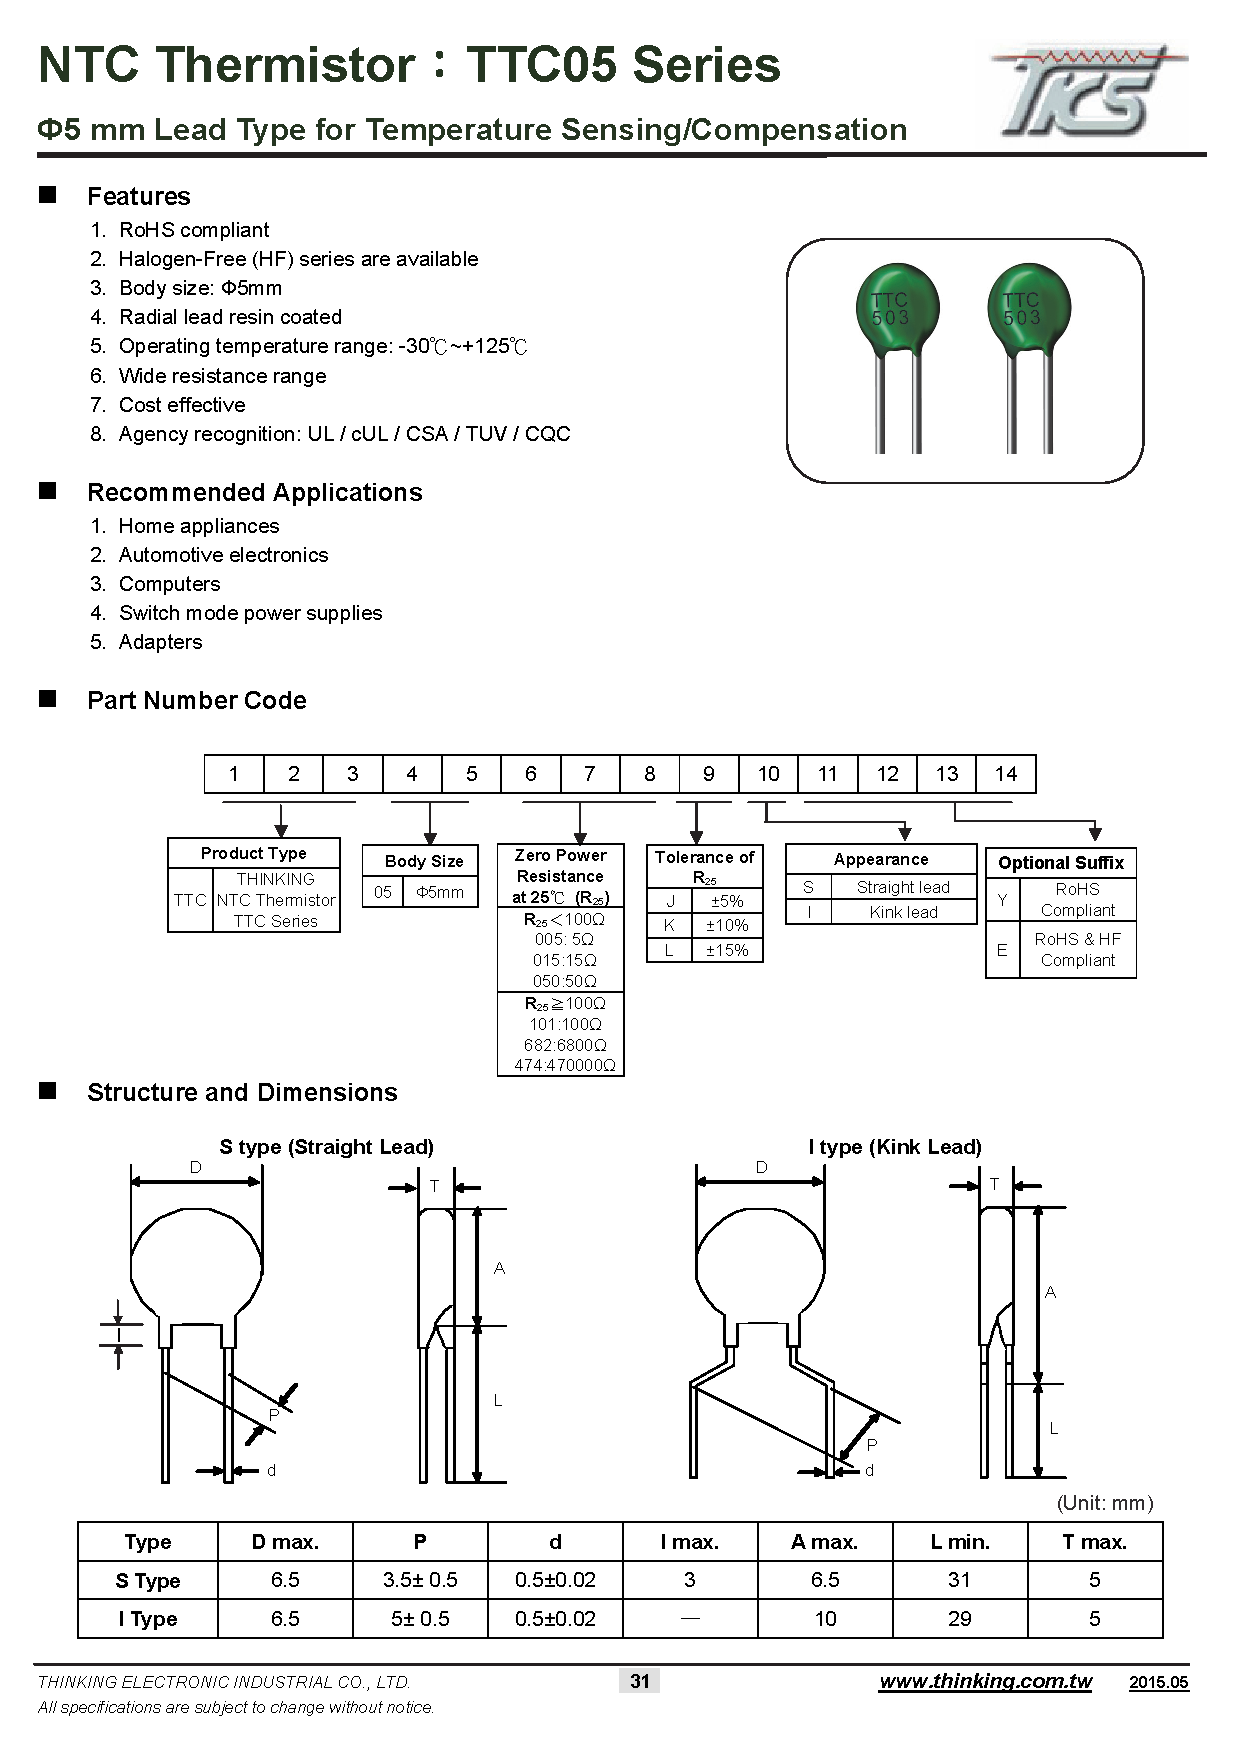
\includepdf{../datasheet/termistor.pdf}

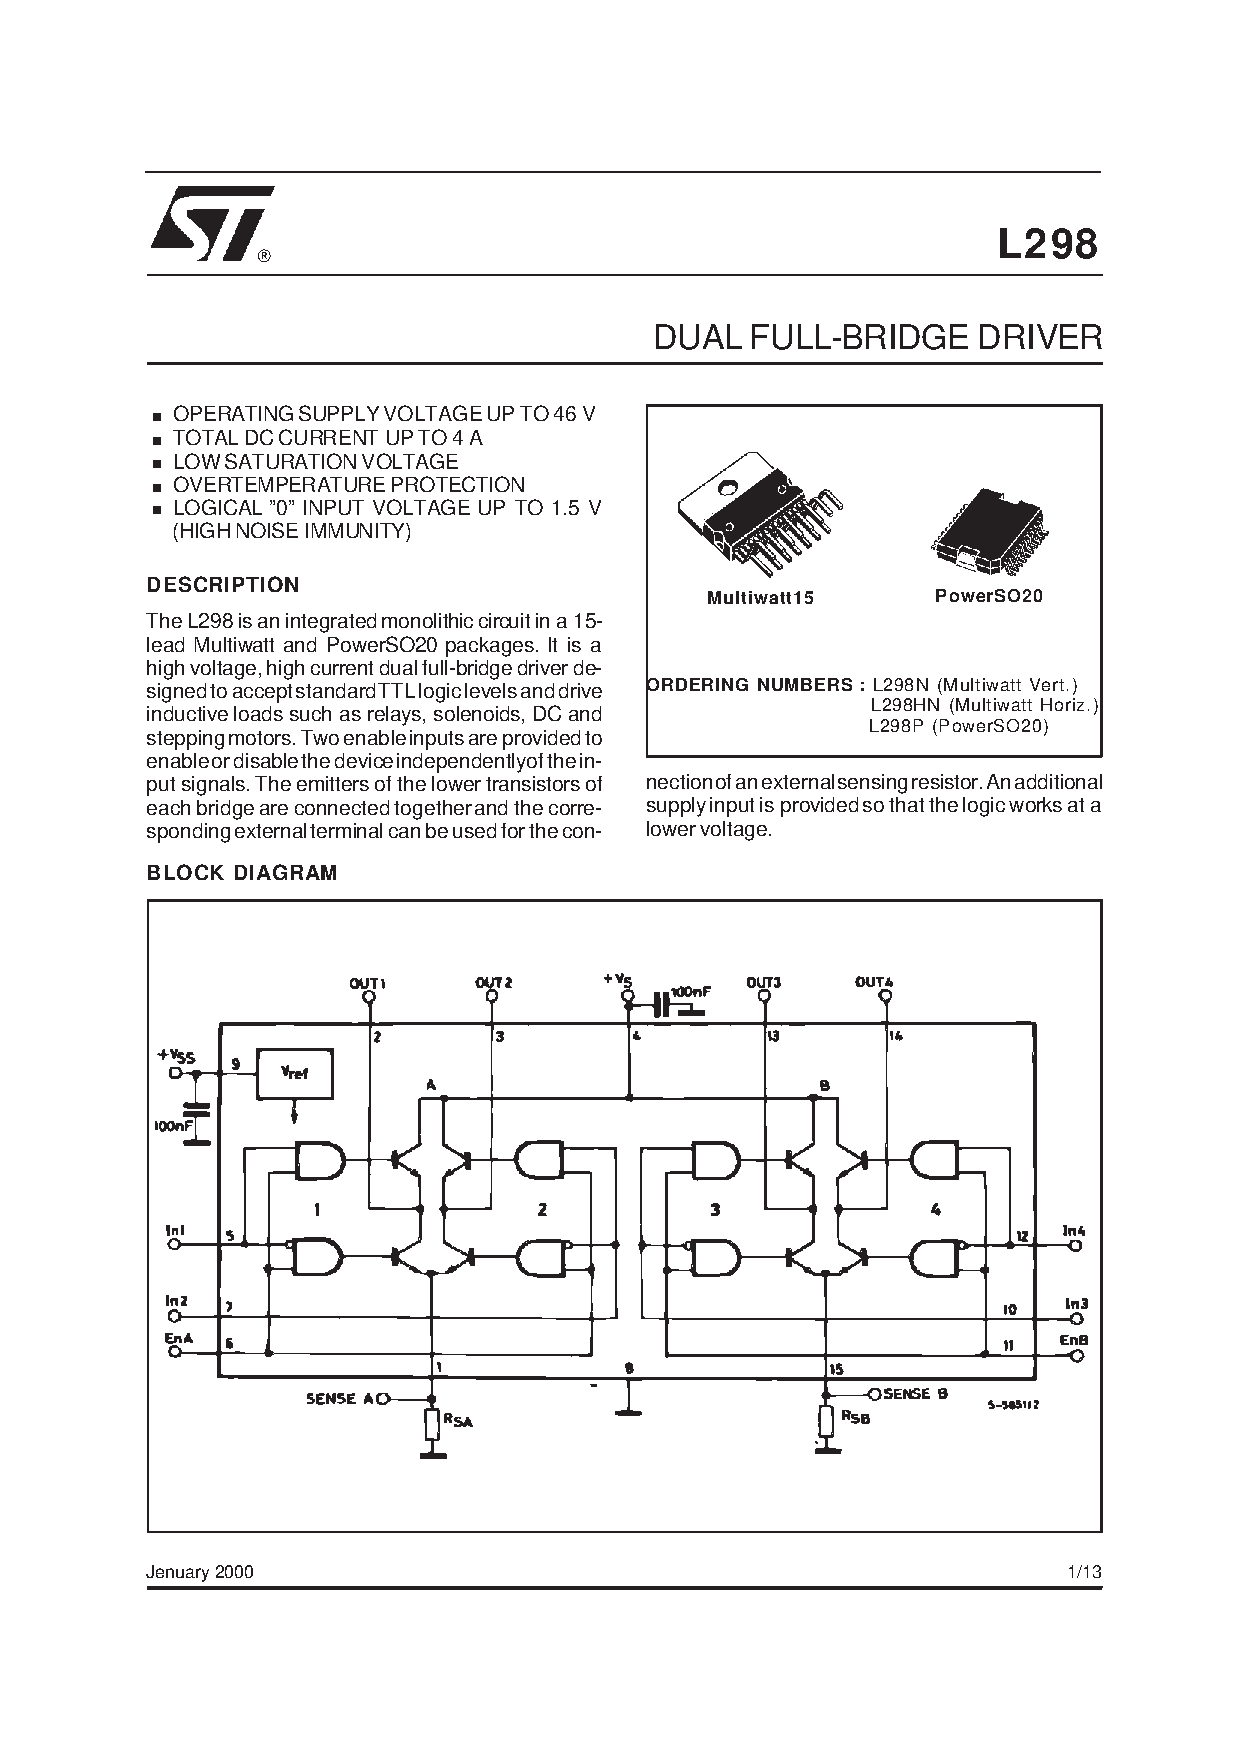
\includepdf[pages={1-7}]{../datasheet/L298.pdf}

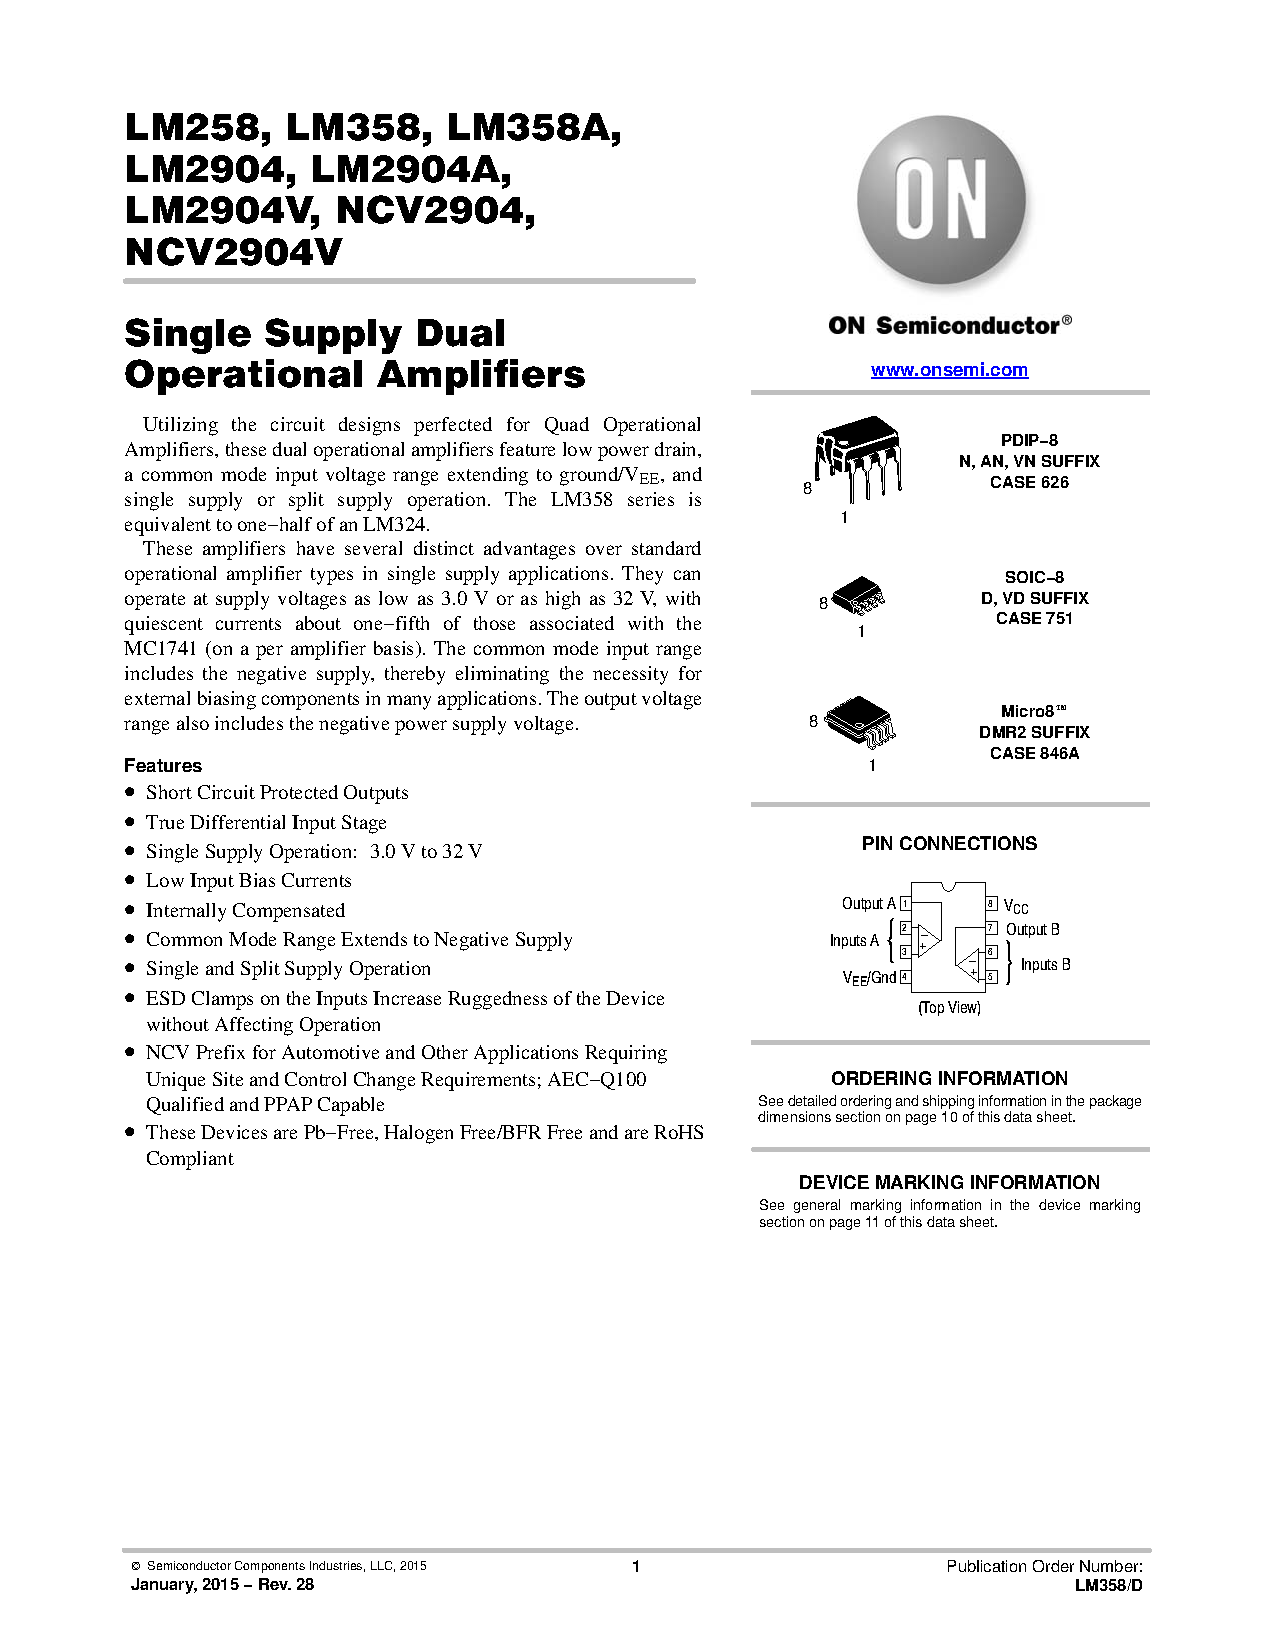
\includepdf[pages={1-2}]{../datasheet/LM358.PDF}

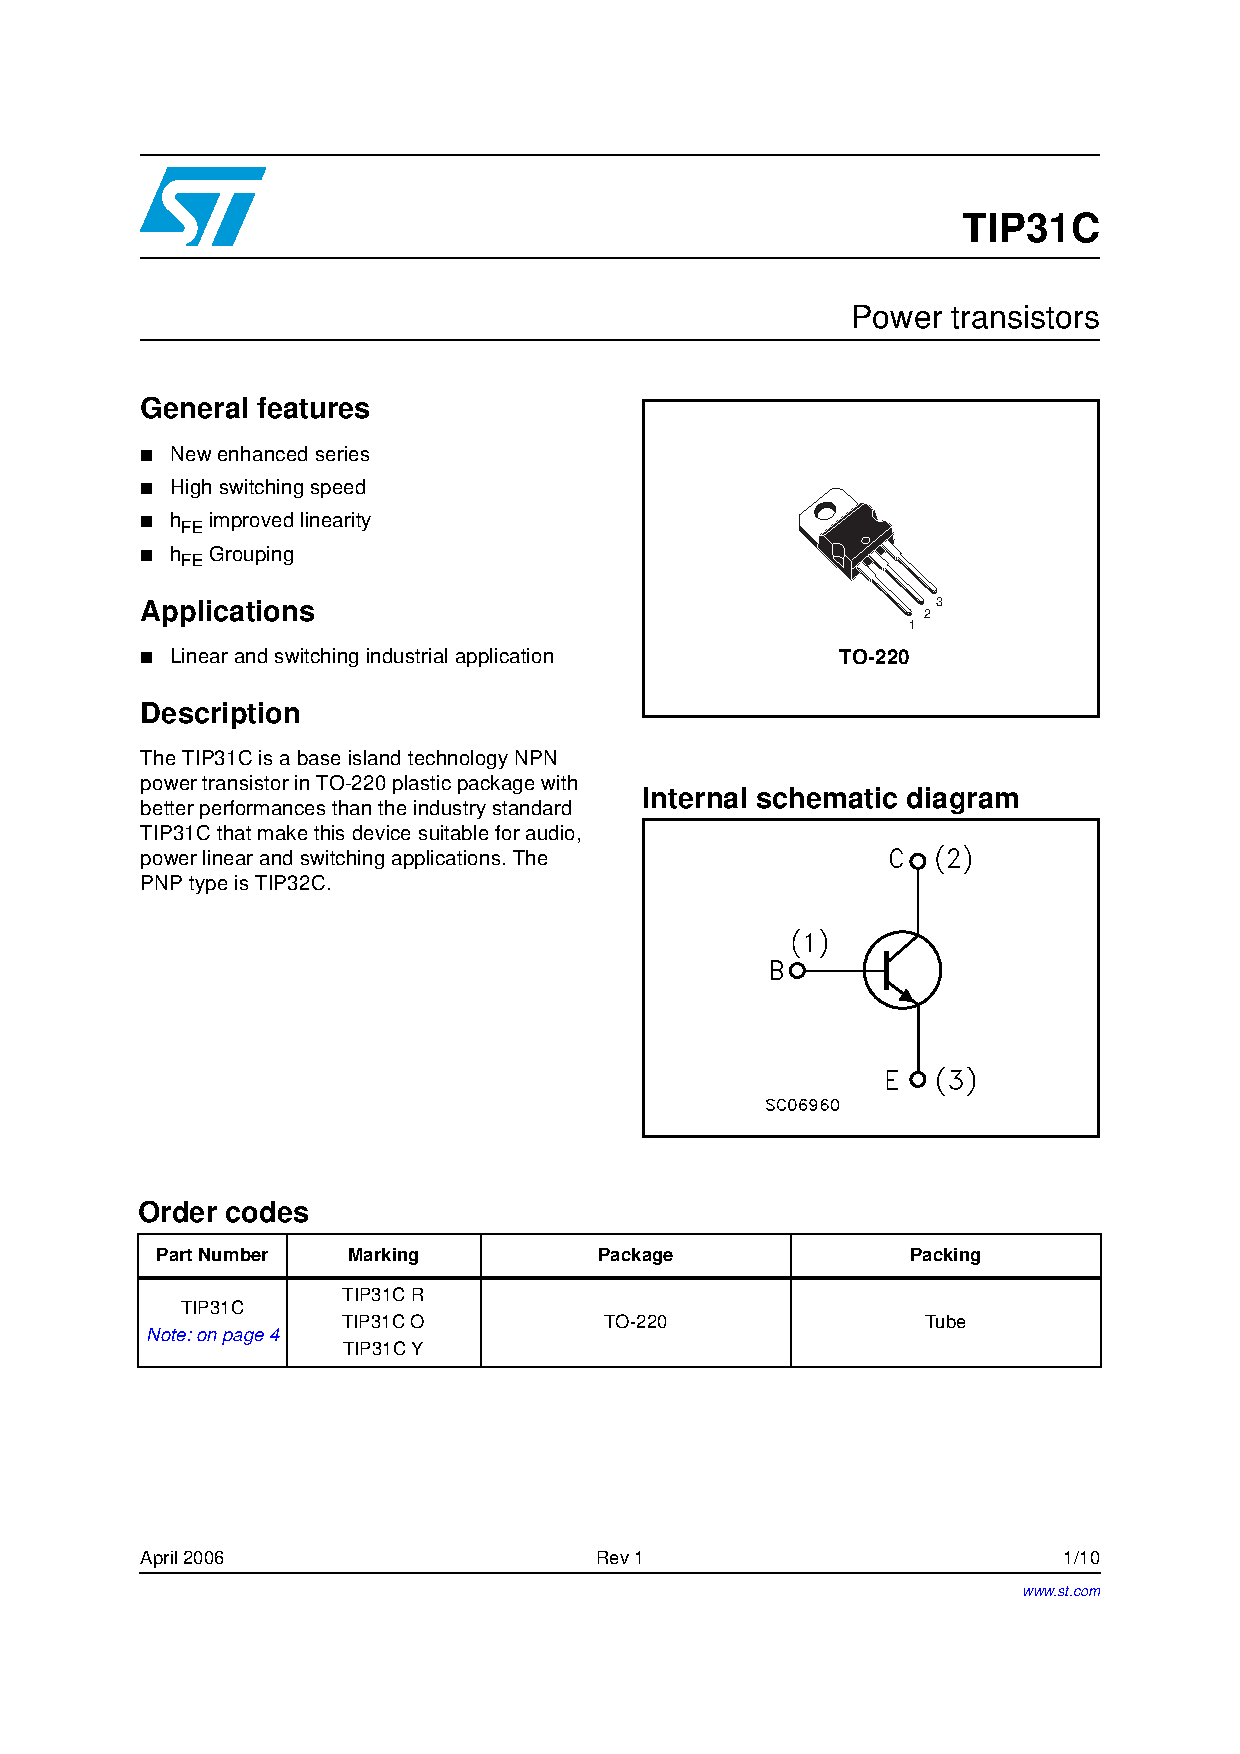
\includepdf[pages={1, 3-4}]{../datasheet/TIP31C.pdf}

\end{document}
